\pdfoutput=1

\documentclass{l4proj}

%
% put any packages here
%

\begin{document}
\title{Are matrix-based or node-linked graphs more readable when representing causal relationships for social and health data?}
\author{Kristina Lazarova}
\date{March, 2017}
\maketitle

\begin{abstract}
We show how to produce a level 4 project report using latex and pdflatex using the 
style file l4proj.cls
\end{abstract}

\educationalconsent
%
%NOTE: if you include the educationalconsent (above) and your project is graded an A then
%      it may be entered in the CS Hall of Fame
%
\tableofcontents
%==============================================================================
\chapter{Literature Review}
\pagenumbering{arabic}

This is the first chapter where I will introduce data visualisation and and explain how I came up with the idea of this research

\chapter{Introduction}
Introduction to the specific area of my research

\chapter{Implementation details}
\section{Software tools and technologies}

Given the opportunity to chose any tools and technologies for the development of this web application was a very exciting task. However, I had to be certain that the right decisions are made. After a research period followed by a trial-error week it was decided that the backend of the application will built with Node.js and JavaScript combined with the web application framework Express. Node.js was chosen on the grounds of being event-driven, non-blocking I/O model which contributes to a very efficient and lightweight software. A Node.js JavaScript engine is also used in the Google Chrome browser. JavaScript servers have incredible performance due to their asynchronous I/O. Node.js appears to be single-threaded from a developer's point of view, as there is no thread management involved in the development process. However, behind the scenes Node.js handles threading, file system events, implements the event loop, feature thread pooling etc. Coming from a Java background, the Maven equivalent in Node.js is NPM. By using NPM commands the developer is able to install variety of different modules to help the implementation process. NPM executes the function of a package manager. Express is the standard server framework for Node.js. It is usually described as a minimal and flexible Node.js web application framework. Many popular frameworks such as KeystoneJS, Kraken and Sails, are built on Express. 

AngularJS 1 was chosen for management of frontend functionality. Even though there is a newer version of the product, the lack of documentation and support online, was a sufficient reason for using the older AngularJS. It uses HTML as a template and enables the developers to extend it to express the application's components clearly. AngularJS supports features such as data binding and dependency injection which decreases the amount of code that a developer would usually write to implement them. 

The database system chosen for the project is PostgreSQL. Considering the size of the project an object-relational database was chosen. In addition, it decided on PostgreSQL in particular because it is open source and has gained a reputation of a reliable database system. Also previous experience with PosgreSQL from developers point of view made the decision easier.

* maybe database schema will be added here *  

 
\section{Challenges}
\begin{verbatim}
		Spring idea failed
		changed to Node.js
		Angular compatibility with Node.js
\end{verbatim}

In the beginning of this project the Java framework Spring was going to be used in the implementation as it is among the most widely used frameworks in industry \cite{shiLuiLi}. This decision was supported by extensive previous experience with Java from developer's point of view and the applicability of the skills to be acquired. However, one of the reasons why Spring is used in industry is because of the large and complex systems that exist there. The Spring framework works on a very high level of abstraction where you can easily write configuration files to add dependencies from different project. Therefore, it is considered rather unfriendly for small independent projects and developers with limited Spring experience. The reasoning behind this conclusion was provoked after a couple of unsuccessful attempts to set relative paths to different CSS and JavaScript files. The issue was found to be in the web application configuration file. This is how the very simple task of reading a css file turned to be a long tedious debugging process after which the realisation that Spring is unnecessary abstract and complex for this project occurred.

A new research for web-application frameworks followed. Node.js backend was chosen because of its event-driven, non-blocking I/O model which creates an efficient and lightweight server-side of the application. Another challenge appeared when trying to incorporate AngularJS with Node.js. Usually in AngularJS one uses curly braces to reference data structure from the AngularJS controller. However, Node.js also uses curly brackets to reference information from the backend in the frontend. After a long research  it was found that Node.js overrides the use of curly braces and the application is not displaying Angular data as it expects it come from the backend. Unfortunately, an appropriate error message does exist and it all had to be discovered during the development process. Instead of using curly brackets one can also use "ng-bind" and achieve the same result. This approached solved the issue until "ng-bind" information was need in "ng-src" to display the appropriate graph image. It is not possible to use "ng-bind" inside "ng-src" so the present solution at the time was no longer solving the problem. Therefore, the Angular configurations had be altered to use a different symbol. Implementing this solved the problem entirely. 


\section{Software reliability testing}

\chapter{Evaluation}
\section{Design}
\section{Participants}
\section{Procedure}
\section{Results}
\section{Discussion}

\chapter{}




\section{First Section in Chapter}
The quick brown fox jumped over the lazy dog.
The quick brown fox jumped over the lazy dog.
The quick brown fox jumped over the lazy dog.
The quick brown fox jumped over the lazy dog.
The quick brown fox jumped over the lazy dog \cite{DIMACS}.
The quick brown fox jumped over the lazy dog.
The quick brown fox jumped over the lazy dog.
The quick brown fox jumped over the lazy dog.
The quick brown fox jumped over the lazy dog.

\subsection{A subsection}
The quick brown fox jumped over the lazy dog.
The quick brown fox jumped over the lazy dog.
The quick brown fox jumped over the lazy dog.
The quick brown fox jumped over the lazy dog.

The quick brown fox jumped over the lazy dog.
The quick brown fox jumped over the lazy dog.
The quick brown fox jumped over the lazy dog.
The quick brown fox \cite{fahle} jumped over the lazy dog.
The quick brown fox jumped over the lazy dog.

\chapter{The Fox and Dog}
The quick brown fox jumped over the lazy dog.
The quick brown fox jumped over the lazy dog.
The quick brown fox jumped over the lazy dog.
The quick brown fox jumped over the lazy dog.
The quick brown fox jumped over the lazy dog.
The quick brown fox jumped over the lazy dog.
The quick brown fox jumped over the lazy dog.
The quick brown fox jumped over the lazy dog.

\section{The Fox Jumps Over}
The quick brown fox jumped over the lazy dog.
The quick brown fox jumped over the lazy dog.
The quick brown fox jumped over the lazy dog.
The quick brown fox jumped over the lazy dog.
The quick brown fox jumped over Uroborus (Figure \ref{uroborus}).
The quick brown fox jumped over the lazy dog.

The quick brown fox jumped over the lazy dog.
The quick brown fox jumped over the lazy dog.
The quick brown fox jumped over the lazy dog.
The quick brown fox jumped over the lazy dog.
The quick brown fox jumped over the lazy dog.
The quick brown fox jumped over the lazy dog.
The quick brown fox jumped over the lazy dog.
The quick brown fox jumped over the lazy dog.
The quick brown fox jumped over the lazy dog.
The quick brown fox jumped over the lazy dog.
The quick brown fox jumped over the lazy dog.

%\vspace{-7mm}
\begin{figure}
\centering
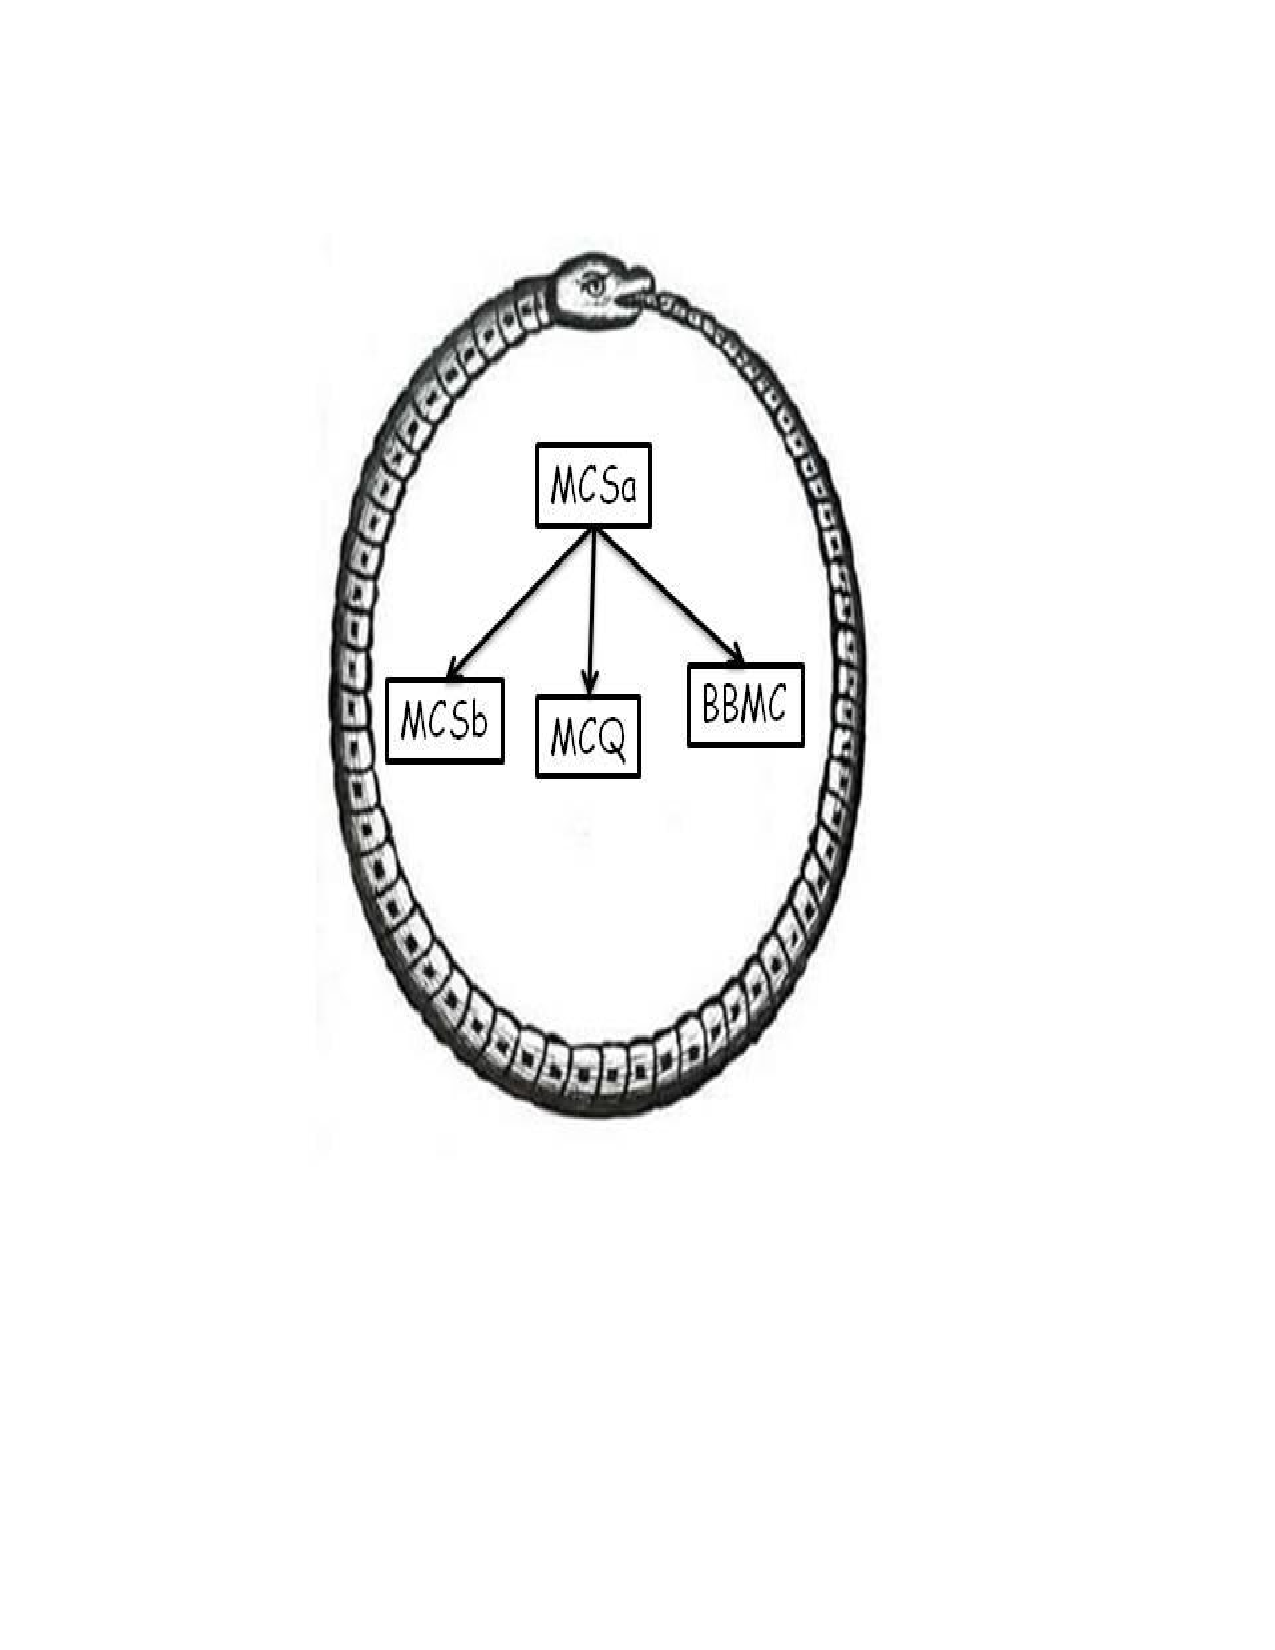
\includegraphics[height=9.2cm,width=13.2cm]{uroboros.pdf}
\vspace{-30mm}
\caption{An alternative hierarchy of the algorithms.}
\label{uroborus}
\end{figure}

The quick brown fox jumped over the lazy dog.
The quick brown fox jumped over the lazy dog.
The quick brown fox jumped over the lazy dog.
The quick brown fox jumped over \cite{ckt} the lazy dog.
The quick brown fox jumped over the lazy dog.
The quick brown fox jumped over the lazy dog.
The quick brown fox jumped over the lazy dog.
The quick brown fox jumped over the lazy dog.

\section{The Lazy Dog}
The quick brown fox jumped over the lazy dog.
The quick brown fox jumped over the lazy dog.
The quick brown fox jumped over the lazy dog.

The quick brown fox jumped over the lazy dog.
The quick brown fox \cite{am97} jumped over the lazy dog.
The quick brown fox jumped over the lazy dog.
The quick brown fox jumped over the lazy dog.
The quick brown fox jumped over the lazy dog.
The quick brown fox jumped over the lazy dog.

%%%%%%%%%%%%%%%%
%              %
%  APPENDICES  %
%              %
%%%%%%%%%%%%%%%%
\begin{appendices}

\chapter{Running the Programs}
An example of running from the command line is as follows:
\begin{verbatim}
      > java MaxClique BBMC1 brock200_1.clq 14400
\end{verbatim}
This will apply $BBMC$ with $style = 1$ to the first brock200 DIMACS instance allowing 14400 seconds of cpu time.

\chapter{Generating Random Graphs}
\label{sec:randomGraph}
We generate Erd\'{o}s-R\"{e}nyi random graphs $G(n,p)$ where $n$ is the number of vertices and
each edge is included in the graph with probability $p$ independent from every other edge. It produces
a random graph in DIMACS format with vertices numbered 1 to $n$ inclusive. It can be run from the command line as follows to produce 
a clq file
\begin{verbatim}
      > java RandomGraph 100 0.9 > 100-90-00.clq
\end{verbatim}
\end{appendices}

%%%%%%%%%%%%%%%%%%%%
%   BIBLIOGRAPHY   %
%%%%%%%%%%%%%%%%%%%%

\bibliographystyle{plain}
\bibliography{bib}

\end{document}
